\documentclass[preprint,5p,times]{elsarticle}

%%%%%%%%%%%%%%   Preample  %%%%%%%%%%%%%%%%%%
%% for comment (texts in between \begin{comment} and \end{comment} will be ignored)
\usepackage{comment} 

%% The amssymb package provides various useful mathematical symbols
\usepackage{amssymb}
%% The amsthm package provides extended theorem environments
\usepackage{amsthm}

%% The lineno packages adds line numbers. Start line numbering with
%% \begin{linenumbers}, end it with \end{linenumbers}. Or switch it on
%% for the whole article with \linenumbers.
\usepackage{lineno}
\linenumbers

%% package for subfigure environment
\usepackage{subcaption}

%% package for type Greek letters without entering into math-mode
\usepackage{textgreek}

%% package for large picture in two-colume
%\usepackage{dblfloatfix}
%\usepackage{fixltx2e}

%% only jpg pdf eps are allowed,tiff format are not allowed in latex
%% eps in principle can't be compiled by pdflatex,pdf not compiled by latex,but Kile can do some intermedate conversion to allow this happen.
\DeclareGraphicsExtensions{.pdf,.eps,.jpg}
%%opening
\journal{NIMA}

\begin{document}

%%%%%%%%%%%%%% Front Matter %%%%%%%%%%%%%%%%%%
\begin{frontmatter}

\title{A versatile PMT test bench and the measurements of 500 Hamamastu R4443-Mod2 phototubes for DAMPE-PSD detector}
%%\title{Title with footnote\tnoteref{t1}}
%%\tnotetext[t1]{FootNote for title}

\author[imp,ucas,lzu]{Yong Zhou}
%\ead{yong@impcas.ac.cn}

\author[imp]{Yuhong Yu}
%%\ead{yuyuhong@impcas.ac.cn}

\author[imp]{Zhiyu Sun\corref{corresponding_author}}
\cortext[corresponding_author]{Corresponding author}
\ead{sunzhy@impcas.ac.cn}

%% Additional Author information %%
%%\author[ano]{Anonymous\fnref{fn1}}
%%\ead{anonymous@anonymous.cn}
%%\fntext[fn1]{FootNote for Anonymous author}

\address[imp]{Institute of Modern Physicas,Chinese Academy of Sciences, 509 Nanchang Road, Lanzhou, 730000, P.R.China}
\address[ucas]{Graduate University of the Chinese Academy of Sciences, 19A Yuquan Road, Beijing, 100049, P.R.China}
\address[lzu]{School of Nuclear Science and Technology, Lanzhou University, 222 South Tianshui Road, Lanzhou, 730000, P.R.China}
%%\address[ano]{Anonymous Address of Anonymous author}

%%
\begin{abstract}
blablabla
\end{abstract}

%%
\begin{keyword}
keyword1
\sep keyword2
\sep keyword3

%% PACS codes here, in the form: \PACS code \sep codes

%% MSC codes here, in the form: \MSC code \sep code
%% or \MSC[2008] code \sep code (2000 is the default)

\end{keyword}

\end{frontmatter}

%%%%%%%%%%%%%%%%  Introduction  %%%%%%%%%%%%%%%%%%%%%%%
\section{Introduction}
\label{sec:introduction}

DArk Matter Paricle Explorer(DAMPE)\cite{Chang_Jin_dampe} is a satellite-borne particle detector for dark matter search and cosmic ray study.
It is designed to cover the energy range from 5~GeV to 10~TeV for electrons and photons with an energy resolution of 1\% at 800~GeV,from 100~GeV to 1~PeV for heavy ions with an energy resolution better than 40\% at 800~GeV.

Plastic scintillator Strip Detector(PSD),which sits at the topmost of the satellite,is a key component of DAMPE detector.
By measuring the energy deposit of particles pentrating through it,PSD serves as a anti-coincidence detector for e/$\gamma$ discrimination as well as a detector for charge measurement up to Z=20.
PSD consists of 82 plastic scintillator strips(EJ-200\cite{ej200}) of dimention $864mm\times28mm\times10mm$,each readout at both ends by a Hamamastu R4443-Mod2 photomultiplier tube.
These strips are arranged into two orthogonally oriented layers,convering an effective area of $820mm\times820mm$.
Each PMT is readout at both dynode 5 and dynode 8 with different gains to cover the large dynamic range from $\sim$0.5~MIPs to $\sim$700~MIPs.
The readout signals are processed by a highly-sensitive ASIC chip(VA32) with the range of 0-14~pC,and then digitized by an ADC with 14~bits resolution.

Unlike groud-based experiments,the power supply system of DAMPE payload can only provide discrete high voltage levels with an interval of 30~V.
Furthermore,every 6 or 7 PMTs of PSD form a HV-group and share the same high voltage channel.
In this case,the ususal method of fine-tuning individual PMT's high voltage to get optimal gain is not available.  
The characteristics of PMTs in the same HV-group should have similar dependency on voltage.
Thus a careful selection of the tubes is mandatory to get uniform energy response across the whole detector and optimal utilization of the mesuring range.
For this selection,the gain of dynode 5 and dynode 8 as a function of supplying voltage needs to be measured precisely.  

On the other hand,the harsh environment of satellite imposes a strict set of quality control processes for the production of PMT modules,as shown in Fig.~\ref{fig:production_procedure}.
A PMT module is composed of a bare PMT tube,baseboards for HV supply and signal readout,silicone rubber for coupling with the palstic scintillator,pouring sealant to protect PMT from vibration and HV breakdown and the supporting Aluminum box.
\begin{figure}[h!]
 \centering
 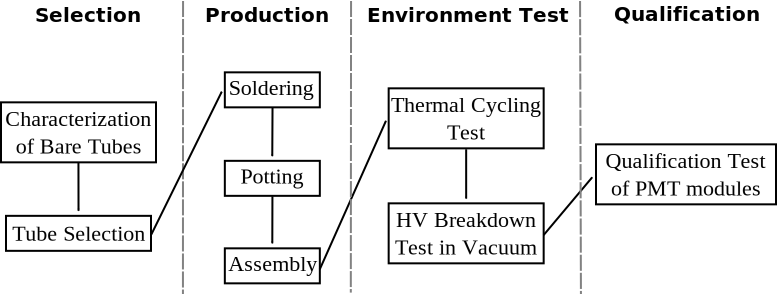
\includegraphics[width=90mm]{pmt_production_procedure}
\caption{Production Procedures of a PMT module.The PMT should be tested during the selection phase and qualification phase}
\label{fig:production_procedure}
\end{figure} 
Some of the PMT modules may get irreversible deterioration,even damage,during these processes.
Thus a qualification test shall be performed to certificate the performance of each PMT module before final installation. 

Considering the large number of tubes involved in the Selection phase and Qualification phase,a PMT test bench for bulk testing was designed and contructed to facilitate this work.
500 bare R4443-Mod2 tubes were thoroughly tested and 200 of them were selected for production and qualification.
Finally,164 PMT modules with the optimal characteristics were installed.
While mainly developped for the DAMPE-PSD project,this test bench has been designed to be as versatile as possible and can be upgaded seamlessly for future experiments.
The detailed description of the test bench will be given in Sec.\ref{sec:description}.Some key characteristics of the test bench is summarized in Sec.\ref{sec:char_testbench}.
The testing results of PSD PMTs and the corresponding selection procedure will be discussed in Sec.\ref{sec:pmt_test}.

%%%%%%%%%%%%%%%% Main Text Body %%%%%%%%%%%%%%%%%%%%%%%
\section{Description of the test bench}
\label{sec:description}

design considerations

schematic diagram and overview of the bench
\begin{figure*}[hb]
 \centering
 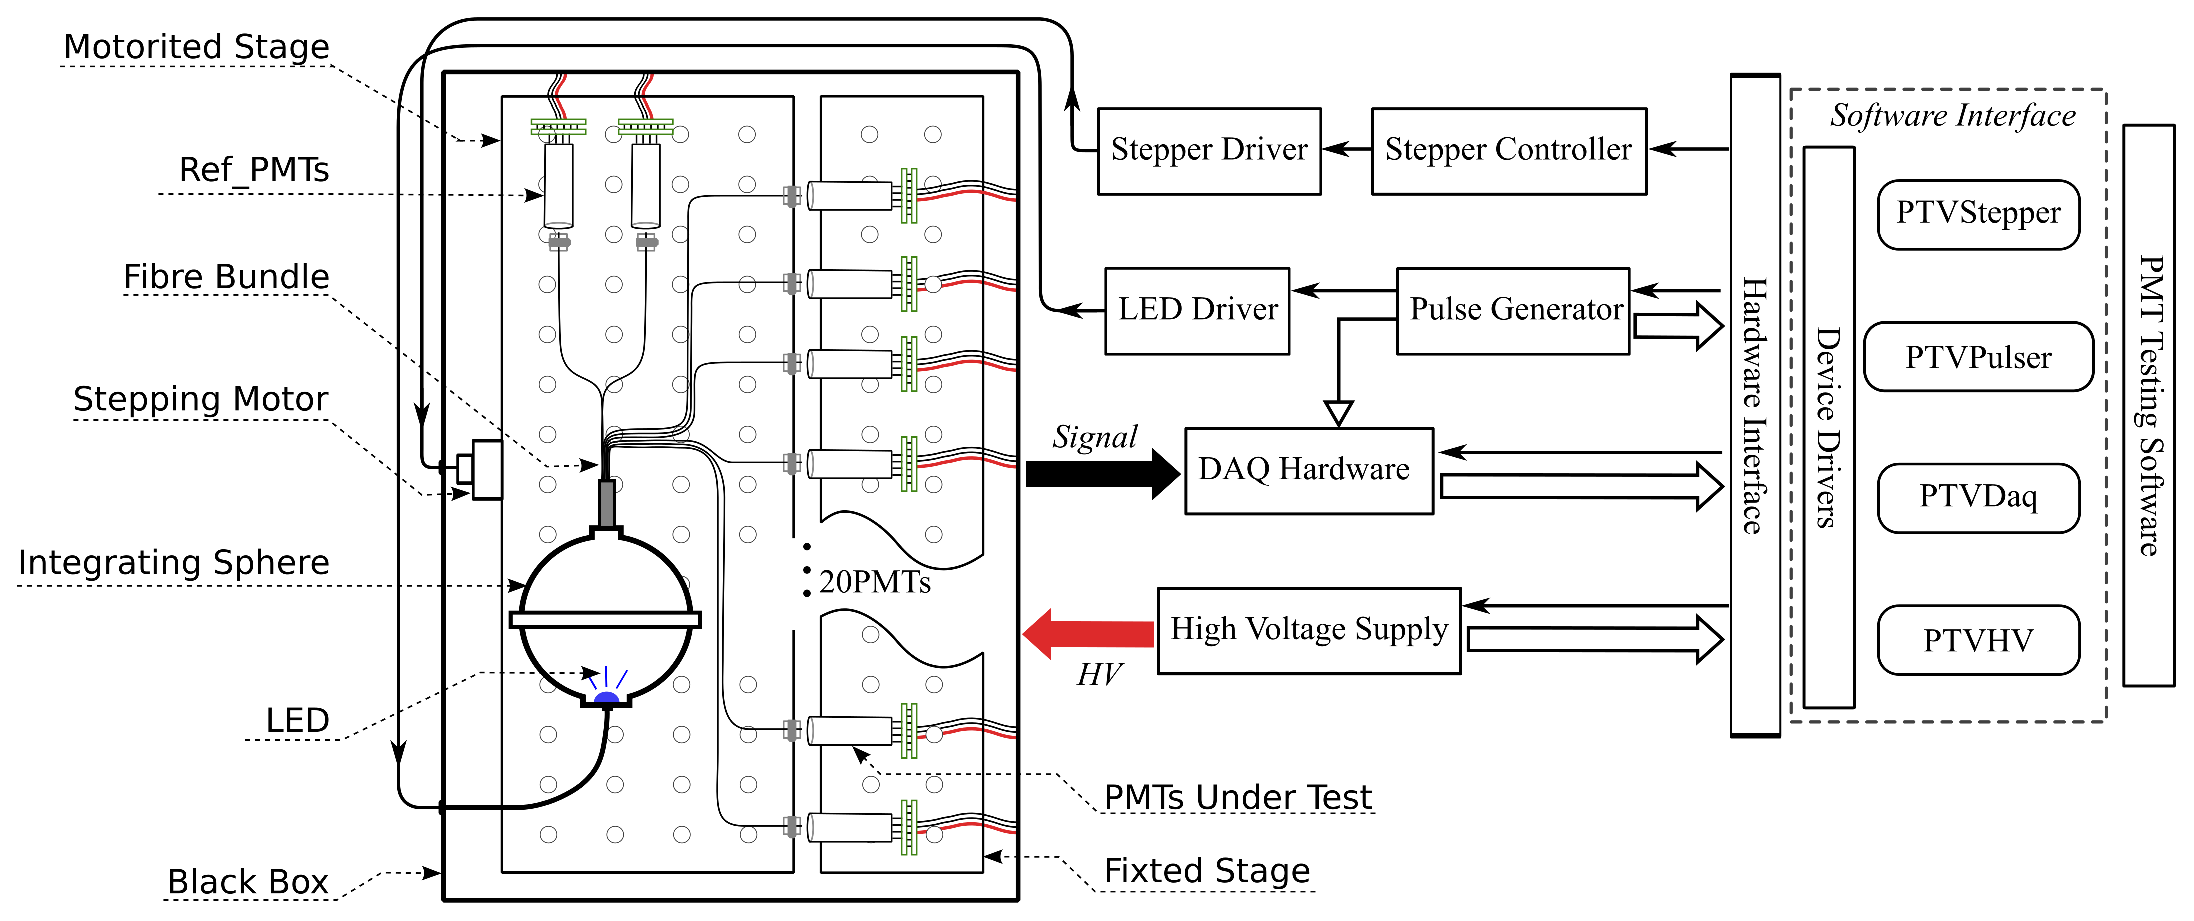
\includegraphics[width=140mm]{testbench_overview}
\caption{Schematic diagram of the PMT test bench system.\textit{PTVStepper},\textit{PTVPulser},\textit{PTVDaq} and \textit{PTVHV} are abstract classes which separate the testing software from the hardware implementation details.}
\label{fig:testbench_overveiw}
\end{figure*} 

summarization of the functionality of the bench,automatic,efficiency

\subsection{Light Source and Distribution}
\label{sec:light_source}

A 3~W blue LED from Z-light\cite{zlight} is apdopted as the light source for the test bench.This product has been used previously as the light source of PMT monitoring and calibration system\cite{yuyuhong_led} 

\subsection{Three-dimention motorized stage}
\label{sec:platform}

A 3~dimention movable platform was built as the supporting structure

\subsection{Auxiliary devices}
\label{sec:integrating_sphere}

\subsection{Reference PMTs}
\label{sec:ref_pmt}

\subsection{Software}
\label{sec:software}
The software system is developped in C++ and run under Windows.
To facilitate maintainence and future upgrade,the software components are groupped in three levels as following:
\begin{enumerate}
 \item Device abstraction,which not only serves as an interface to the underlying hardwares,but also handles the abstraction of different types of devices. 
 \item Framework libraries,which defines a general testing procedure and provides utility classes for configuration and management.
 \item User inerface,which provides command line based or graphical executables for user interaction. 
\end{enumerate}

Designed as a versatile equipment,different hardware modules may be used in the future.
For example,while the general-purpose VME or CAMAC platform may meet the demands of most of the use cases,some experiments may prefer to use project-specific DAQ hardware for testing.
In another case,a laser light source with a ultra-short pulsing driver may be used for time-related characterization.
%Instead of developping a dedicated program each time a hardware interface changes,an abstraction of the devices is adoptted to separate the testing procedure from hardware implementation details.
Abstract classes for stepper controller,light pulser,DAQ system and HV supplier are defined,as shown in Fig.\ref{fig:testbench_overveiw}.
Common operations of each type of device are extracted and encapsulated in the corresponding abstract class,which are the only interface to high level software components.
Concrete classes inheritted from the same abstract class represent different devices of the same type.
Currently,the concrete classes for Leetro MPC07SP motion controller,Tektronix AFG3252 pulse generator,CAEN SY1527 power supply system and DAMPE DAQ board are implemented.
An DAQ interface for the CAMAC system based on CC-USB controller is also implemented and thoroughly tested.

Built upon the abstract device inerface,a general testing framework is defined,as shown in Fig.\ref{fig:software_framework}.
\begin{figure}[h!]
\centering
 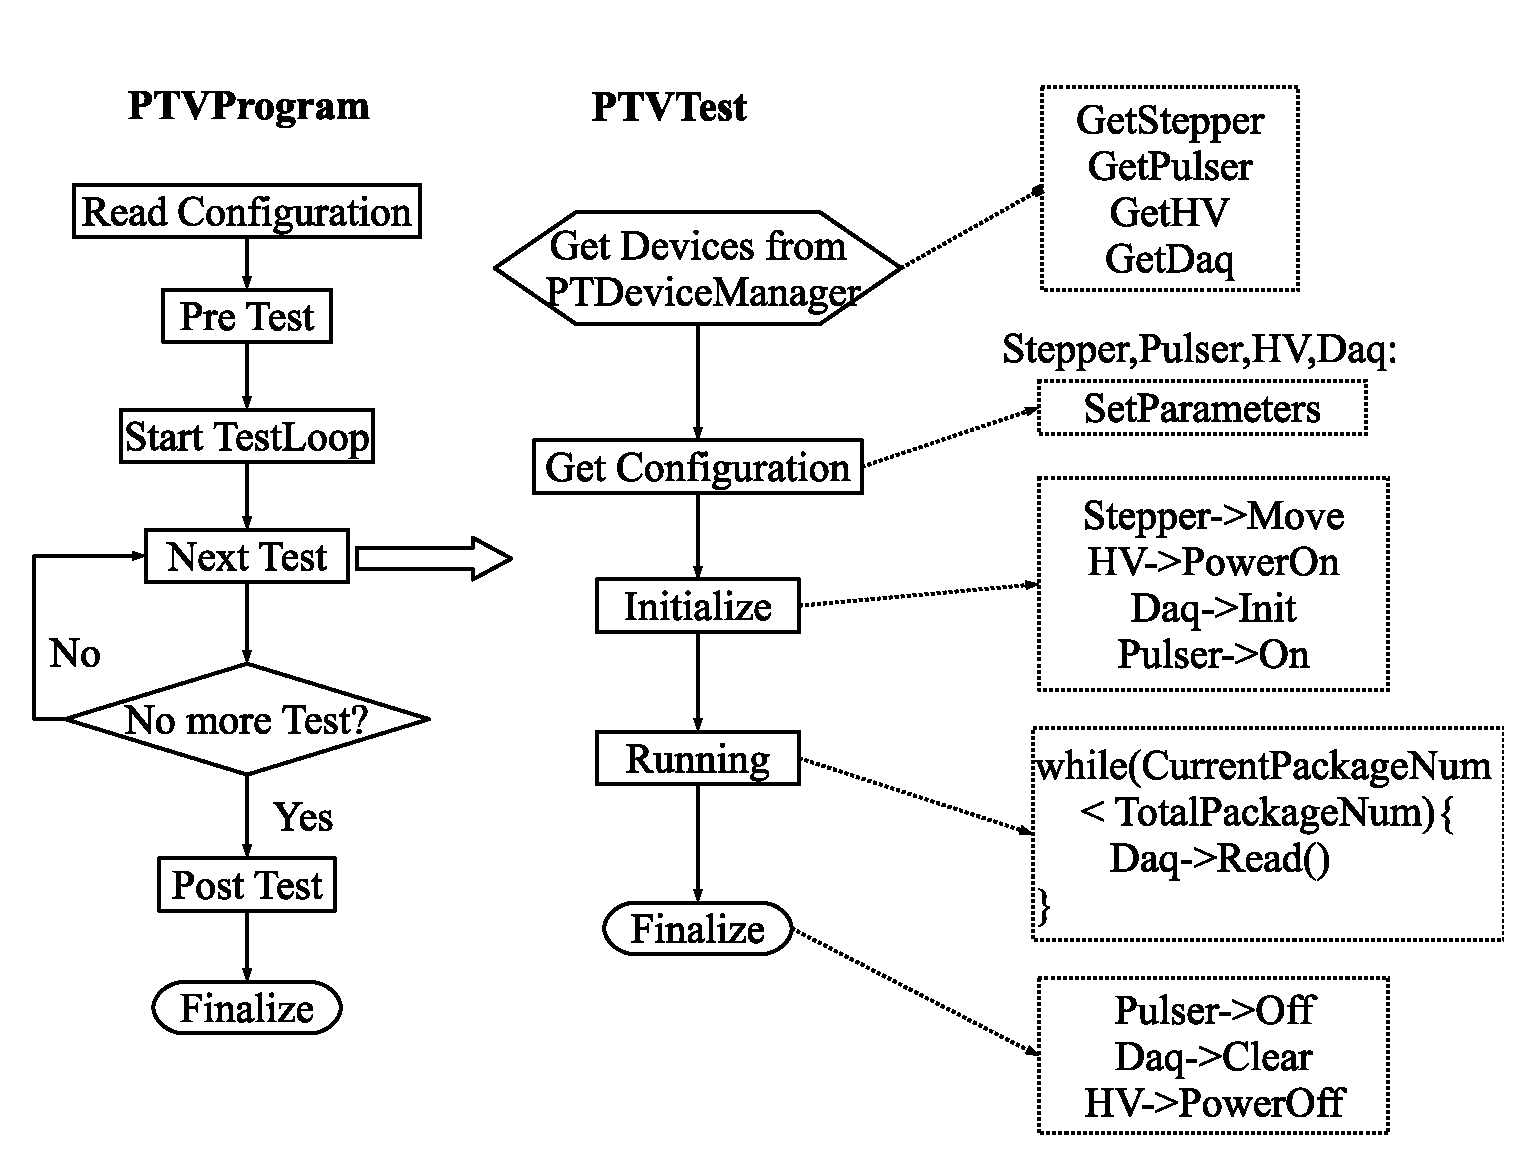
\includegraphics[width=90mm]{software_framework}
\caption{Software framework}
\label{fig:software_framework}
\end{figure}
A \textit{PTVProgram} represents the measurement procedure for a specific characteristic of PMT,such as cathode uniformity,gain,dark count rate,and so on.
A \textit{PTVTest} represents the real testing operation,which corresponds to a specific testing condition.
Usually,a \textit{PTVProgram} is consist of multiple \textit{PTVTest}.
For example,for cathode uniformity test,the stepping motor will move to a series of positions.
At each position,the PMT response will be recorded.
Here the 
As a first step,all used concrete device classes will be registered in the singlton class \textit{PTDeviceManager} and then retrieved from it during testing. 

Two testing programs are defined for DAMPE projects,one for pedestal testing and one for amplitude scan and voltage scan.
The warming step is defined in the PreTest phase of amplitude and voltage scan program.

Based on the framework library,a light-weight user interface based on PDCurses\cite{pdcurses} has been developped.
This program also incorporates status monitoring function,which is developped utilizing Phtread-win32 library\cite{pthread_win32}.

A dedicated analysis program based on ROOT libraries is also developped for the DAMPE PSD project.
The program does not depends on the framework libraries described above.
The analysis results are inserted into a database for easy query.
\section{Characteristics of the test bench}
\label{sec:char_testbench}

\subsection{Long-term Stability}
\label{sec:longterm_stability}

\subsection{Spatial Uniformity of Integrating Sphere}
\label{sec:spatialuniformity_insph}

\subsection{Transmission Uniformity of Fibre-bundle}
\label{sec:transuniformity_fibre}

\section{PMT testing for PSD}
\label{sec:pmt_test}

\subsection{Selection criteria}
\label{sec:selection}

\subsection{Testing Result of Relative Gain}
\label{sec:relative_gain}

\subsection{Testing Result of Dynode Ratio}
\label{sec:dynode_ratio}

\subsection{PMT Qualification}
\label{sec:qualification}

%%%%%%%%%%%%%%%%  Conclustion   %%%%%%%%%%%%%%%%%%%%%%%
\section{Conclusions}
\label{sec:conclustions}

%%%%%%%%%%%%%%%% Acknowledgement %%%%%%%%%%%%%%%%%%%%%%%
\section*{Acknowledgement}

%%%%%%%%%%%%%%%%    Appendix     %%%%%%%%%%%%%%%%%%%%%%%
%% The Appendices part is started with the command \appendix;
%% appendix sections are then done as normal sections
\appendix
\section{}
\label{app:}

%%%%%%%%%%%%%%%%   Bibliography  %%%%%%%%%%%%%%%%%%%%%%%
%% bibliography style
\section*{References}
\bibliographystyle{elsarticle-num}

%% From BibTex file
\bibliography{mybib}

%% From hand-writing
\begin{comment}
%%\begin{thebibliography}{00}

%%\bibitem{CEBAF12}
%%V.D. Burkert, \emph{arXiv:1203.2373v1 [nucl-ex]}, 2012.

%%\bibitem{CLAS}
%%B.A. Mecking \emph{et al.}, Nucl. Ins. and Meth. in Phys. Research {\bf A503} (2003) 513

%%\end{thebibliography}
\end{comment}

\end{document}
\endinput